% Transcription littérale du TD 09.
% Les abréviations et l'ordre des raisonnements de la copie sont conservés.

\exercise{5}{}

\begin{statementbox}
5| Soit $E$ le $\R$-ev des fonctions lipschitziennes : $[0, 1] \to \R$ [$f \in E$ ssi $\exists k \in \R_+ / \forall (x, y) \in [0, 1]^2, |f(x) - f(y)| \leq k|x - y|$] Pour $f \in E$, on définit
\[ K(f) := \sup \left\{ \frac{|f(x) - f(y)|}{|x - y|}, x \neq y \in [0, 1]^2 \right\} \]
\begin{enumerate}[label=\alph*)]
  \item Mq $N : E \to \R, f \mapsto |f(0)| + K(f)$ est une norme sur $E$.
  \item Mq $N$ et $N_\infty$ (ie : $\forall f \in E, N_\infty(f) := \sup_{t \in [0, 1]} |f(t)|$) ne sont pas équivalentes.
  \item Mq $N$ est équivalente à $N' : E \to \R, f \mapsto N_\infty(f) + K(f)$.
\end{enumerate}
\end{statementbox}

\begin{solution}
\partanswer{a)}
Soit $f \in E$ et $k \geq 0$ / $f$ est $k$-lipschitzienne, alors $\forall (x, y) \in [0, 1]^2 / x \neq y$, $\frac{|f(x) - f(y)|}{|x - y|} \leq k$ donc $K(f)$ est bien défini et $K(f) \leq k$.
Si $N(f) = 0$ alors $|f(0)| = 0 = K(f)$ et $\forall t \in ]0, 1], f(t) = f(0) = 0$. Donc $f = 0$.
Soit $\lambda \in \R$ et $f \in E$, $N(\lambda f) = |\lambda f(0)| + \underbrace{K(\lambda f)}_{= |\lambda| K(f)} = |\lambda| N(f)$.
Soient $(f, g) \in E^2$.
$N(f + g) = |(f + g)(0)| + K(f + g) \leq |f(0)| + |g(0)| + K(f + g)$.
Soient $x \neq y \in [0, 1]^2$, on a :
\[ |(f + g)(x) - (f + g)(y)| \leq |f(x) - f(y)| + |g(x) - g(y)| \leq (K(f) + K(g)) \times |x - y| \]
Donc $f + g \in E$ et $K(f + g) \leq K(f) + K(g)$. Donc $N(f + g) \leq N(f) + N(g)$.

\partanswer{b)}
Soit $f \in E$ et $t \in ]0, 1]$. $|f(t)| \leq |f(0)| + \underbrace{|f(t) - f(0)|}_{\leq t K(f) \leq K(f)} \leq N(f)$ et c'est vrai aussi pour $t = 0$. D'où $N_\infty(f) \leq N(f)$.
De plus, si $f$ est $\mathcal{C}^1 : [0, 1] \to \R$, l'inégalité des accroissements finis implique que $K(f) \leq \sup_{t \in [0, 1]} |f'(t)|$, et $\forall t_0 \in [0, 1[, \forall h \neq 0, \left|\frac{f(t_0 + h) - f(t_0)}{h}\right| \leq K(f)$, d'où lorsque $h \to 0$, $|f'(t_0)| \leq K(f)$ (et par continuité en $1$, $|f'(1)| \leq K(f)$). Finalement, si $f$ est $\mathcal{C}^1$, $K(f) = \sup_{t \in [0, 1]} |f'(t)| = N_\infty(f')$.

Soit pour $n \in \N, f_n : [0, 1] \to \R, t \mapsto t^n \in E$, on a : $\forall n \in \N^*, N_\infty(f_n) = 1$ et $N_\infty(f'_n) = n = K(f_n)$ ($N(f_n) = n \xrightarrow[n \to +\infty]{} +\infty$).
Ainsi, $(f_n)_{n \in \N}$ est bornée pour $N_\infty$ mais pas pour $N$. Donc $N_\infty$ et $N$ ne sont pas équivalentes.

\partanswer{c)}
On a vu que $N_\infty \leq N$, donc $\forall f \in E, N'(f) \leq N(f) + \underbrace{K(f)}_{\leq N(f)} \leq 2 N(f)$.
Réciproquement, soit $f \in E$ :
\[ N(f) = |f(0)| + K(f) \leq N_\infty(f) + K(f) \leq N'(f) \]
Donc $N$ et $N'$ sont équivalentes.
\end{solution}

\exercise{9}{}

\begin{statementbox}
9| Soit $G$ un sous-groupe de $GL_n(\C)$, on suppose que $G$ est un voisinage de $I_n$ (pour une norme quelconque), mq $G = GL_n(\C)$.
\end{statementbox}

\begin{solution}
$\exists \varepsilon_0 > 0 / B_{\|\cdot\|_\infty}(I_n, \varepsilon_0) \subset G$. On munit $\mathcal{M}_n(\C)$ de $\|M = (m_{i,j})_{1 \leq i, j \leq n}\|_\infty = \max_{1 \leq i, j \leq n} |m_{i,j}|$.
\begin{itemize}
  \item Soit $i \neq j, \lambda \in \C$. $\forall k \in \N^*, T_{i,j}\left(\frac{\lambda}{k}\right)^k = T_{i,j}(\lambda)$ (car $\forall (\lambda, \mu) \in \C^2, T_{i,j}(\lambda + \mu) = T_{i,j}(\lambda) \times T_{i,j}(\mu)$).
  Or $\lim_{k \to +\infty} \frac{\lambda}{k} = 0$ donc $\exists k_0 \in \N^* / \forall k \geq k_0, \left|\frac{\lambda}{k}\right| < \varepsilon_0$, alors $\left\|T_{i,j}\left(\frac{\lambda}{k_0}\right) - I_n\right\|_\infty < \varepsilon_0$ et $T_{i,j}\left(\frac{\lambda}{k_0}\right) \in G$. Donc $T_{i,j}(\lambda) = T_{i,j}\left(\frac{\lambda}{k_0}\right)^{k_0} \in G$ (par stabilité par produit).
  \item Soit $j \in \llbracket 1, n \rrbracket$ et $\alpha \in \C^*$ avec $\alpha = \rho e^{i\theta}$, $\rho = |\alpha| > 0$ et $\theta \in [0, 2\pi[$.
  Soit $k \in \N^*, \rho^{\frac{1}{k}} e^{\frac{i\theta}{k}} \xrightarrow[k \to +\infty]{} 1$. Donc $\exists k_0 \in \N^*, \left|\rho^{\frac{1}{k_0}} e^{\frac{i\theta}{k_0}} - 1\right| < \varepsilon_0$.
  $\left\|D_j\left(\rho^{\frac{1}{k_0}} e^{\frac{i\theta}{k_0}}\right) - I_n\right\|_\infty < \varepsilon_0$, d'où $D_j\left(\rho^{\frac{1}{k_0}} e^{\frac{i\theta}{k_0}}\right) \in G$, et $D_j(\alpha) = D_j\left(\rho^{\frac{1}{k_0}} e^{\frac{i\theta}{k_0}}\right)^{k_0}$ [car $D_j(\alpha \beta) = D_j(\alpha) D_j(\beta) \; \forall (\alpha, \beta) \in (\C^*)^2$].
  $D_j(\alpha) \in G$ par stabilité par produit.
\end{itemize}
Or toute matrice inversible est produit de matrices de transvection et de dilatation, donc comme $G$ est un sous-groupe, $GL_n(\C) \subset G$ et $\boxed{GL_n(\C) = G}$.

\begin{remarkbox}
Rem : Si on suppose seulement $\mathring{G} \neq \emptyset$ ie : $\exists M_0 \in G, \exists \varepsilon_0 > 0, B_{\|\cdot\|_{op}}(M_0, \varepsilon_0) \subset G$.
Soit $\|\cdot\|$ une norme sur $\C^n$, nous verrons que $\|M\|_{op} = \sup_{\substack{X \in \mathcal{M}_{n,1}(\C) \\ X \neq 0}} \frac{\|MX\|}{\|X\|}$ est une norme d'algèbre [ie : sous-multiplicative] sur $\mathcal{M}_n(\C)$.
Soit $M \in \mathcal{M}_n(\C)$, on a : $\|M - M_0\|_{op} = \|(M M_0^{-1} - I_n) M_0\|_{op} \leq \|M M_0^{-1} - I_n\|_{op} \times \|M_0\|_{op}$.
Donc si $\|M M_0^{-1} - I_n\|_{op} < \frac{\varepsilon_0}{\|M_0\|_{op}}$ alors $\|M - M_0\|_{op} < \varepsilon_0$ et $M \in G$.
Alors $\forall M' \in \mathcal{M}_n(\C)$, si $\|M' - I_n\|_{op} < \frac{\varepsilon_0}{\|M_0\|_{op}}$, alors $\underbrace{M' M_0}_{\in G} \in G$ donc $M' = (M' M_0) M_0^{-1} \in G$. Donc $B_{\|\cdot\|_{op}}\left(I_n, \frac{\varepsilon_0}{\|M_0\|_{op}}\right) \subset G$ et d'après ce qui précède, $GL_n(\C) = G$.
\end{remarkbox}
\end{solution}

\exercise{37}{}

\begin{statementbox}
37| Soit $E$ un $\mathbb{K}$-evn.
\begin{enumerate}[label=\alph*)]
  \item Soit $A \neq \emptyset \subset E$ ; mq $\forall x \in E, d_A(x) = d_{\overline{A}}(x)$. En déduire que pour $A, B$ deux parties $\neq \emptyset$ de $E$ : $\overline{A} = \overline{B}$ ssi $d_A = d_B$ [où $\forall x \in E, d_A(x) = d(x, A) := \inf \{\|x - a\| / a \in A\}$].
  \item Soit $(A, B)$ deux parties $\neq \emptyset$ de $E$ ; on définit :
  \[ \rho(A, B) := \sup_{x \in E} |d_A(x) - d_B(x)| \quad (\in \R \cup \{+\infty\}) \quad \text{et} \quad \alpha(A, B) := \max \left\{ \sup_{a \in A} d_B(a), \sup_{b \in B} d_A(b) \right\} \]
  Mq $\rho(A, B) = \alpha(A, B)$.
\end{enumerate}
\end{statementbox}

\begin{solution}
\partanswer{a)}
Soit $x \in E$, comme $A \subset \overline{A}$, $d_{\overline{A}}(x) := \inf \{\|x - a'\| / a' \in \overline{A}\} \leq d_A(x)$.
Soit $\varepsilon > 0$, $\exists a' \in \overline{A}, \|x - a'\| < d_{\overline{A}}(x) + \varepsilon$, et par définition de $\overline{A}$, $\exists a \in A, \|a - a'\| < \varepsilon$.
Alors $d_A(x) \leq \|x - a\| \leq \|x - a'\| + \|a - a'\| < d_{\overline{A}}(x) + 2\varepsilon$, et ceci valant pour tout $\varepsilon > 0$, alors $d_A(x) \leq d_{\overline{A}}(x)$. D'où $d_A = d_{\overline{A}}$.
\begin{itemize}
  \item Si $\overline{A} = \overline{B}$, alors $d_A = d_{\overline{A}} = d_{\overline{B}} = d_B$.
  \item Si $d_A = d_B$, alors $\overline{A} = \{x \in E / d_A(x) = 0\} = d_A^{-1}(\{0\}) = d_B^{-1}(\{0\}) = \overline{B}$.
\end{itemize}
On a bien $d_A = d_B$ ssi $\overline{A} = \overline{B}$.

\partanswer{b)}
Soit $a \in A$, alors $d_A(a) = 0$ et $d_B(a) = |d_A(a) - d_B(a)| \leq \rho(A, B)$.
Donc $\sup_{a \in A} d_B(a) \leq \rho(A, B)$ (éventuellement $+\infty$). De même, $\sup_{b \in B} d_A(b) \leq \rho(A, B)$, d'où $\alpha(A, B) \leq \rho(A, B)$.

Si $\alpha(A, B) = +\infty$, on a (dans $\R \cup \{+\infty\}$) $\rho(A, B) \leq \alpha(A, B)$.
Supposons désormais que $\alpha(A, B) < +\infty$.
Soit $x \in E$ ; on veut mq $|d_A(x) - d_B(x)| \leq \alpha(A, B)$. Cela équivaut à $\begin{cases} d_A(x) - d_B(x) \leq \alpha(A, B) \\ \text{et } d_B(x) - d_A(x) \leq \alpha(A, B) \end{cases}$.
Comme $\alpha(A, B) = \alpha(B, A)$, il suffit de mq $d_A(x) - d_B(x) \leq \alpha(A, B)$, ie : $d_A(x) \leq \alpha(A, B) + d_B(x)$.
Soit $\varepsilon > 0$ : $\exists b \in B / \|x - b\| \leq d_B(x) + \varepsilon$ et $b$ étant fixé, $\exists a \in A / \|a - b\| < d_A(b) + \varepsilon \leq \alpha(A, B) + \varepsilon$.
Il vient : $d_A(x) \leq \|x - a\| \leq \|a - b\| + \|x - b\| \leq \alpha(A, B) + d_B(x) + 2\varepsilon$.
Ceci valant $\forall \varepsilon > 0, d_A(x) \leq \alpha(A, B) + d_B(x)$. Ainsi, $\forall x \in E : |d_A(x) - d_B(x)| \leq \alpha(A, B)$, donc $\rho(A, B) \leq \alpha(A, B)$.
Ainsi $\boxed{\rho(A, B) = \alpha(A, B)}$.

\begin{remarkbox}
Rem : $\rho(A, B) = 0$ ssi $\forall x \in E, d_A(x) = d_B(x)$ ssi, d'après a), $\overline{A} = \overline{B}$.
\end{remarkbox}
\end{solution}

\exercise{3}{}

\begin{statementbox}
3| Soit $E := \{f : \R \to \R \text{ continue, bornée}\}$ (sev de $\mathcal{C}^0(\R, \R)$).
\begin{enumerate}[label=\alph*)]
  \item Soit $p \in \N$, mq on peut définir $N_p : E \to \R, f \mapsto N_p(f)$ avec $N_p(f) = \sup_{t \in \R} (|f(t)| |t|^p e^{-|t|})$ et que c'est une norme sur $E$.
  \item Mq pour $p \neq q$, $N_p$ et $N_q$ ne sont pas équivalentes.
\end{enumerate}
\end{statementbox}

\begin{solution}
\partanswer{a)}
Soit $f \in E, \forall t \in \R, |f(t)| \leq \|f\|_\infty$, d'où $|f(t)| |t|^p e^{-|t|} \leq \|f\|_\infty |t|^p e^{-|t|}$.
Soit $\varphi_p : t \mapsto |t|^p e^{-|t|}$ paire.
$\varphi_p$ est $\mathcal{C}^1$ sur $\R_+$ (pour $p \geq 1$) et $\forall t > 0, \varphi'_p(t) = t^{p-1} e^{-t} (p - t)$.
\[
\begin{array}{c|ccccc}
t & 0 & & p & & +\infty \\ \hline
\varphi'_p(t) & & + & 0 & - & \\ \hline
\varphi_p(t) & 0 & \nearrow & \varphi_p(p) & \searrow & 0
\end{array}
\qquad \varphi_p(p) = \|\varphi_p\|_\infty.
\]
Donc $N_p(f) \leq \|f\|_\infty \|\varphi_p\|_\infty < +\infty$.
Soit $f \in E$ telle que $N_p(f) = 0$. Alors : $\forall t \in \R^*, f(t) = 0$ (car $|t|^p e^{-|t|} > 0$). Par continuité de $f$, $f(0) = 0$, donc $f = 0$.
Soit $\lambda \in \R$, $N_p(\lambda f) = \sup_{t \in \R} (|\lambda| |f(t)| |t|^p e^{-|t|}) = |\lambda| N_p(f)$ (voir lemme de cours).
Soient $f, g \in E$. $\forall t \in \R, |(f + g)(t)| |t|^p e^{-|t|} \leq |f(t)| |t|^p e^{-|t|} + |g(t)| |t|^p e^{-|t|} \leq N_p(f) + N_p(g)$.
Par minimalité, $N_p(f + g) \leq N_p(f) + N_p(g)$.
Donc $N_p$ est une norme.

\partanswer{b)}
Soit $p \in \N$ et $q \in \N$ avec $p \neq q$.
Pour $n \in \N$, posons $f_n : \R \to \R, t \mapsto e^{-n|t|} \in E$.
$g_n : t \mapsto f_n(t) |t|^p e^{-|t|} = |t|^p e^{-(n+1)|t|}$ paire et $\mathcal{C}^1$ sur $\R_+^*$.
$\forall t > 0, g'_n(t) = t^{p-1} e^{-(n+1)t} (p - (n+1)t)$ (pour $p \geq 1$ ; pour $p = 0$, le maximum est atteint en $0$).
\[
\begin{array}{c|ccccc}
t & 0 & & \frac{p}{n+1} & & +\infty \\ \hline
g'_n(t) & & + & 0 & - & \\ \hline
g_n(t) & 0 & \nearrow & & \searrow & 0
\end{array}
\]
$N_p(f_n) = \left(\frac{p}{n+1}\right)^p e^{-p} = p^p e^{-p} \times \frac{1}{(n+1)^p}$.
Supposons $p < q$.
$N_q((n+1)^q f_n) = q^q e^{-q}$.
$N_p((n+1)^q f_n) = p^p e^{-p} (n+1)^{q-p} \xrightarrow[n \to +\infty]{} +\infty$.
Ainsi $((n+1)^q f_n)_n$ est bornée pour $N_q$ mais pas pour $N_p$.
Donc $N_p$ et $N_q$ ne sont pas équivalentes.
\end{solution}

\exercise{41}{}

\begin{statementbox}
41| Soit $(n, p) \in (\N^*)^2$ et $f \in \mathcal{L}(\R^n, \R^p)$.
Montrer l'équivalence : $\underbrace{(f \text{ est surjective})}_{\text{(i)}}$ ssi $\underbrace{(\forall \mathcal{O} \text{ ouvert de } \R^n, f(\mathcal{O}) \text{ est un ouvert de } \R^p)}_{\text{(ii)}}$.
\end{statementbox}

\begin{solution}
Supposons (ii) : Alors $\operatorname{Im}(f) = f(\R^n)$ est un sev ouvert dans $\R^p$, donc d'intérieur $\neq \emptyset$, d'où $\operatorname{Im} f = \R^p$ donc $f$ est surjective. D'où (ii) $\implies$ (i).

Supposons (i) : On a donc $n \geq p$. Soit $(e_1, \dots, e_p) \in (\R^p)^p$ la base canonique de $\R^p$, qu'on munit de $\left\|\sum_{j=1}^p y_j e_j\right\|' = \max_{1 \leq j \leq p} |y_j|$. $\forall j \in \llbracket 1, p \rrbracket, \exists \varepsilon_j \in \R^n / f(\varepsilon_j) = e_j$.
Soit $(\alpha_1, \dots, \alpha_p) \in \R^p$, si $\sum_{j=1}^p \alpha_j \varepsilon_j = 0$ alors : $f\left(\sum_{j=1}^p \alpha_j \varepsilon_j\right) = \sum_{j=1}^p \alpha_j e_j = 0$ or $(e_1, \dots, e_p)$ est libre donc $\forall j \in \llbracket 1, p \rrbracket, \alpha_j = 0$. Donc $(\varepsilon_1, \dots, \varepsilon_p)$ est libre.
On la complète en une base $(\varepsilon_1, \dots, \varepsilon_p, \dots, \varepsilon_n)$ de $\R^n$ / $(\varepsilon_{p+1}, \dots, \varepsilon_n)$ est une base de $\operatorname{Ker} f$, qu'on munit de $\left\|\sum_{i=1}^n x_i \varepsilon_i\right\| = \max_{1 \leq i \leq n} |x_i|$ [car si $x \in \operatorname{Vect}(\varepsilon_1, \dots, \varepsilon_p) \cap \operatorname{Ker} f$, $x = \sum_{j=1}^p x_j \varepsilon_j$ et $f(x) = 0 = \sum_{j=1}^p x_j e_j$, $x = 0$].
Soit $\mathcal{O}$ un ouvert non vide de $\R^n$, et $y_0 \in f(\mathcal{O})$, $\exists x_0 \in \mathcal{O} / f(x_0) = y_0$.
Donc il existe $r_0 \in \R_+^*$ tq $B_{\|\cdot\|}(x_0, r_0) \subset \mathcal{O}$. Soit $y \in B_{\|\cdot\|'}(y_0, r_0)$.
$y = \underbrace{y_0}_{f(x_0)} + \sum_{j=1}^p \alpha_j e_j$ avec $\forall j \in \llbracket 1, p \rrbracket, |\alpha_j| < r_0$.
$= f\left(x_0 + \sum_{j=1}^p \alpha_j \varepsilon_j\right)$ et $\left\|x_0 - \left(x_0 + \sum_{j=1}^p \alpha_j \varepsilon_j\right)\right\| = \max_{1 \leq j \leq p} |\alpha_j| < r_0$.
Donc $\left(x_0 + \sum_{j=1}^p \alpha_j \varepsilon_j\right) \in \mathcal{O}$. Donc $y \in f(\mathcal{O})$ d'où (i) $\implies$ (ii) (car $B_{\|\cdot\|'}(y_0, r_0) \subset f(\mathcal{O})$).
\end{solution}

\exercise{58}{}

\begin{statementbox}
58| Soit $P \in \C[X]$, $\mathcal{F}$ fermé de $\C$ ; mq $P(\mathcal{F})$ est fermé.
\end{statementbox}

\begin{solution}
\begin{itemize}
  \item Si $P$ est constant $= z_0$, si $\mathcal{F} \neq \emptyset, P(\mathcal{F}) = \{z_0\}$ est fermé (et si $\mathcal{F} = \emptyset, P(\mathcal{F}) = \emptyset$ est fermé).
  \item Sinon, soit $(z'_n)_{n \in \N} \in P(\mathcal{F})^\N / \lim_{n \to +\infty} z'_n = z' \in \C$. $\forall n \in \N, \exists z_n \in \mathcal{F} / P(z_n) = z'_n$.

  \textbf{Lemme :} Si $P \in \C[X]$ non constant, $\lim_{|z| \to +\infty} |P(z)| = +\infty$. \\
  \textbf{Dém :} Si $P = a_0 + a_1 X + \dots + a_m X^m$, $m \geq 1, a_m \neq 0$. $\forall z \in \C^*, P(z) = a_m z^m \underbrace{\left(1 + \frac{a_{m-1}}{a_m z} + \dots + \frac{a_0}{a_m z^m}\right)}_{\to 1 \text{ quand } |z| \to +\infty}$.
  D'où $P(z) \underset{|z| \to +\infty}{\sim} a_m z^m$ et $|P(z)| \sim |a_m| |z|^m \xrightarrow[|z| \to +\infty]{} +\infty$.

  Si $(z_n)_{n \in \N}$ n'était pas bornée, on pourrait extraire $(z_{\sigma(n)})_{n \in \N} / \lim_{n \to +\infty} |z_{\sigma(n)}| = +\infty$.
  Alors, d'après le lemme : $\lim_{n \to +\infty} \underbrace{|z'_{\sigma(n)}|}_{|P(z_{\sigma(n)})|} = +\infty$ ce qui ne se peut car $(z'_n)_{n \in \N}$ converge.
  Ainsi, $(z_n)_{n \in \N}$ est bornée, on peut extraire $z_{\varphi(n)} \xrightarrow[n \to +\infty]{} z \in \C$, comme $\mathcal{F}$ est fermé, $z \in \mathcal{F}$.
  Comme $P$ est continue, $\lim_{n \to +\infty} \underbrace{P(z_{\varphi(n)})}_{z'_{\varphi(n)}} = z' = P(z) \in P(\mathcal{F})$, donc $z' \in P(\mathcal{F})$.
\end{itemize}
\end{solution}

\exercise{8}{}

\begin{statementbox}
8| Soit $E = \mathcal{C}^1([0, 1], \R)$.
On définit $\forall f \in E, N(f) = \sqrt{f^2(0) + \int_0^1 {f'}^2}$.
Mq c'est une norme sur $E$ et que $\|\cdot\|_\infty \leq \sqrt{2} N$. Sont-elles équivalentes ?
\end{statementbox}

\begin{solution}
Soit $\varphi : E^2 \to \R, (f, g) \mapsto f(0)g(0) + \int_0^1 f' g'$. $\varphi$ est une forme bilinéaire symétrique.
Soit $f \in E$, $\varphi(f, f) = f^2(0) + \int_0^1 {f'}^2 \geq 0$.
Si $\varphi(f, f) = 0$ alors $f^2(0) = 0$ donc $f(0) = 0$, et $\int_0^1 {f'}^2 = 0$ donc $\forall t \in [0, 1], {f'}^2(t) = 0$, puis $f'(t) = 0$, $f$ est constante donc $f = 0$.
$\varphi$ est donc un produit scalaire et $N$ est une norme.

Soit $f \in E, \forall t \in [0, 1]$ :
\[ |f(t)| \leq |f(0)| + \int_0^t |f'| \leq |f(0)| + \int_0^1 |f'| \underset{\text{C-S}}{\leq} |f(0)| + \sqrt{\int_0^1 1^2} \sqrt{\int_0^1 {f'}^2} \]
D'où $|f(t)| \leq |f(0)| + \sqrt{\int_0^1 {f'}^2}$ et $\|f\|_\infty \leq |f(0)| + \sqrt{\int_0^1 {f'}^2}$.

\textbf{Lemme :} $\forall (a, b) \in {\R_+}^2, a + b \leq \sqrt{2}\sqrt{a^2 + b^2}$. \\
\textbf{Dém :} $(a + b)^2 = a^2 + b^2 + 2ab$, $(\sqrt{2}\sqrt{a^2 + b^2})^2 = 2a^2 + 2b^2$, et $2a^2 + 2b^2 - (a + b)^2 = a^2 + b^2 - 2ab = (a - b)^2 \geq 0$. Donc $a + b \leq \sqrt{2}\sqrt{a^2 + b^2}$.

D'où avec le lemme :
\[ |f(0)| + \sqrt{\int_0^1 {f'}^2} \leq \sqrt{2}\sqrt{f^2(0) + \int_0^1 {f'}^2} \]
et $\|\cdot\|_\infty \leq \sqrt{2} N$.

Soit pour $n \in \N, f_n : [0, 1] \to \R, t \mapsto t^n \in E$.
On a $\int_0^1 {f'_n}^2 = \int_0^1 (n t^{n-1})^2 \, dt = n^2 \frac{1}{2n - 1}$ (pour $n \geq 1$).
$\|f_n\|_\infty = 1$ et $N(f_n) \xrightarrow[n \to +\infty]{} +\infty$.
Ainsi $N$ et $\|\cdot\|_\infty$ ne sont pas équivalentes.
\end{solution}

\exercise{32}{}

\begin{statementbox}
32| Soit $S$ un ensemble infini, $E = \mathcal{B}(S, \R)$ (bornée de $S$ dans $\R$) muni de $\|\cdot\|_\infty$.
Mq il n'existe pas de partie de $E$ à la fois dénombrable et dense.
$\big[$On pourra considérer, pour $X \subset S : \mathbf{1}_X : S \to \R, x \mapsto 1 \text{ si } x \in X, x \mapsto 0 \text{ sinon}$, et pour $(X, Y) \in \mathcal{P}(S)^2$ avec $X \neq Y$, évaluer $\|\mathbf{1}_X - \mathbf{1}_Y\|_\infty$.$\big]$
\end{statementbox}

\begin{solution}
Pour $(X, Y) \in \mathcal{P}(S)^2$ avec $X \neq Y$ : $\forall x \in S, \underbrace{|\mathbf{1}_X(x) - \mathbf{1}_Y(x)|}_{\in \{0, 1, -1\}} \leq 1$, et $\exists x \in (X \setminus Y) \cup (Y \setminus X)$ alors $|\mathbf{1}_X(x) - \mathbf{1}_Y(x)| = 1$. Donc $\|\mathbf{1}_X - \mathbf{1}_Y\|_\infty = 1$.

Par inégalité triangulaire $B\left(\mathbf{1}_X, \frac{1}{2}\right) \cap B\left(\mathbf{1}_Y, \frac{1}{2}\right) = \emptyset$.
$\big[$s'il existe $f \in B\left(\mathbf{1}_X, \frac{1}{2}\right) \cap B\left(\mathbf{1}_Y, \frac{1}{2}\right)$, $1 = \|\mathbf{1}_X - \mathbf{1}_Y\|_\infty \leq \|\mathbf{1}_X - f\|_\infty + \|\mathbf{1}_Y - f\|_\infty < 1$ ce qui ne se peut.$\big]$

S'il existe $A \subset E$ dénombrable et dense :
$\forall X \subset S, \exists f_X \in A / f_X \in B\left(\mathbf{1}_X, \frac{1}{2}\right)$ par densité.
Et ce qui précède mq $\varphi : \mathcal{P}(S) \to A, X \mapsto f_X$ est injective, ce qui n'est pas ($\mathcal{P}(S)$ est non dénombrable).
\end{solution}

\exercise{38}{}

\begin{statementbox}
38| Soit $A := \left\{ \left(\frac{1}{n} + \frac{1}{p}\right)^{n+p} \;\middle/\; (n, p) \in {\N^*}^2 \right\}$. Déterminer $\overline{A}$.
\end{statementbox}

\begin{solution}
\begin{center}
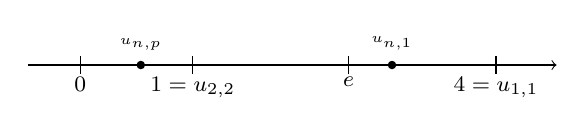
\begin{tikzpicture}[scale=1.1]
  \draw[->] (-0.6,0) -- (5.5,0);
  \draw (0,-0.1) -- (0,0.1) node[below=4pt] {\footnotesize $0$};
  \draw (1.3,-0.1) -- (1.3,0.1) node[below=4pt] {\footnotesize $1 = u_{2,2}$};
  \draw (3.1,-0.1) -- (3.1,0.1) node[below=4pt] {\footnotesize $e$};
  \draw (4.8,-0.1) -- (4.8,0.1) node[below=4pt] {\footnotesize $4 = u_{1,1}$};
  \filldraw (0.7,0) circle (1.2pt) node[above=2pt] {\tiny $u_{n,p}$};
  \filldraw (3.6,0) circle (1.2pt) node[above=2pt] {\tiny $u_{n,1}$};
\end{tikzpicture}
\end{center}

Soit $n \in \N^*$, $u_{n,1} = \left(1 + \frac{1}{n}\right)^{n+1} = \exp\left((n+1)\ln\left(1 + \frac{1}{n}\right)\right) = \exp\left(-(n+1)\ln\left(\frac{n}{n+1}\right)\right)$ (avec $\frac{n}{n+1} = 1 - \frac{1}{n+1}$).
Comme pour $x > -1$, $\ln(1 + x) \leq x$, on a $u_{n,1} \geq e$.
De plus $\ln\left(1 + \frac{1}{n}\right) = \frac{1}{n} + o\left(\frac{1}{n}\right)$, $(n+1)\ln\left(1 + \frac{1}{n}\right) \xrightarrow[n \to +\infty]{} 1$, et $\lim_{n \to +\infty} u_{n,1} = e$.
Donc $e \in \overline{A}$.

Si $n \geq 2$ et $p \geq 2$, $\frac{1}{n} + \frac{1}{p} \leq 1$ et $u_{n,p} \leq 1$.
De plus $u_{n,n} = \left(\frac{2}{n}\right)^{2n} \xrightarrow[n \to +\infty]{} 0$.
Donc $0 \in \overline{A}$ et $A \cup \{0, e\} \subset \overline{A}$.

Soit $x \in \R \setminus (A \cup \{0, e\})$ :
\begin{itemize}
  \item si $x > e$ : comme $\lim_{n \to +\infty} u_{n,1} = e$, $\exists n_0 \in \N^* / \forall n \geq n_0, e \leq u_{n,1} \leq \frac{e + x}{2}$ (et si $n \geq 2, p \geq 2, u_{n,p} \leq 1 < e$). Comme $x \notin A$, $x \notin \overline{A}$.
  \item si $x \in ]1, e[$ : $d(x, A) \geq \min\{x - 1, e - x\} > 0$, donc $x \notin \overline{A}$.
  \item de même si $x < 0$ ($x \notin \overline{A}$).
  \item si $x \in ]0, 1[$ : soit $(n, p) \in {\N^*}^2$ avec $n \geq 2$ et $p \geq 2$ ($u_{2,2} = 1$ et si $(n, p) \neq (2, 2)$, $u_{n,p} \leq \left(\frac{1}{2} + \frac{1}{3}\right)^{n+p} = \left(\frac{5}{6}\right)^{n+p}$).
  Si par exemple $n \geq p$, $u_{n,p} \leq \left(\frac{5}{6}\right)^{n+1} \xrightarrow[n \to +\infty]{} 0$.

  \begin{center}
  \begin{tikzpicture}[scale=1.0]
    \draw (0,0) -- (3.5,0);
    \draw (0,-0.1) -- (0,0.1) node[below=4pt] {\footnotesize $0$};
    \draw (0.9,-0.1) -- (0.9,0.1) node[below=4pt] {\footnotesize $\frac{x}{2}$};
    \draw (1.8,-0.1) -- (1.8,0.1) node[above=2pt] {\footnotesize $x \notin A$};
    \draw (3.5,-0.1) -- (3.5,0.1) node[below=4pt] {\footnotesize $1$};
  \end{tikzpicture}
  \end{center}

  $\exists n_1 \in \N^* / \forall n \geq n_1, \left(\frac{5}{6}\right)^{n+1} < \frac{x}{2}$, et sinon $p \geq n_1, u_{n,p} < \frac{x}{2}$.
  Donc si $u_{n,p} \in \left[\frac{x}{2}, 1\right]$, nécessairement $n < n_1$ et $p < n_1$.
  Il n'y en a qu'un nombre fini.
  Donc $x \notin \overline{A}$.
\end{itemize}
Finalement : $\boxed{\overline{A} = A \cup \{0, e\}}$.
\end{solution}

\exercise{46}{}

\begin{statementbox}
46| (Th de Mazur-Ulam)
Soit $(E, \|\cdot\|_E)$ et $(F, \|\cdot\|_F)$ des $\R$-evn, $T$ une isométrie surjective de $E \to F$ [ie $\forall (x, y) \in E^2, \|T(x) - T(y)\|_F = \|x - y\|_E$].
On veut mq $T$ est affine.
\begin{enumerate}[label=\alph*)]
  \item Soit $f : E \to F / \forall (x, x') \in E^2, f\left(\frac{x + x'}{2}\right) = \frac{f(x) + f(x')}{2}$. Mq $f$ est affine, ie $g : E \to F, x \mapsto f(x) - f(0)$ est linéaire.
  \item Soit $(a, b) \in E^2$, on définit $B_1 := \left\{ x \in E \;\middle/\; \|x - a\| = \|x - b\| = \left\|\frac{b - a}{2}\right\| \right\}$ et par récurrence sur $n \in \N^*$,
  \[ B_{n+1} = \left\{ x \in B_n \;\middle/\; \forall y \in B_n, \|x - y\| \leq \frac{\delta(B_n)}{2} \right\} \]
  Mq $\forall n \in \N^*, B_n \neq \emptyset$, borné et symétrique par rapport à $\frac{a + b}{2}$ [ie $\forall x \in B_n, a + b - x \in B_n$].
  Justifier que $\lim_{n \to +\infty} \delta(B_n) = 0$.
  En déduire que $\bigcap_{n \in \N^*} B_n = \left\{\frac{a + b}{2}\right\}$.
  \item Mq $T\left(\frac{a + b}{2}\right) = \frac{T(a) + T(b)}{2}$, conclure.
\end{enumerate}
\end{statementbox}

\begin{solution}
\partanswer{a)}
On a $g(0) = 0$.
Et pour $(x, x') \in E^2$ :
\[ g\left(\frac{x + x'}{2}\right) = f\left(\frac{x + x'}{2}\right) - f(0) = \frac{f(x) - f(0)}{2} + \frac{f(x') - f(0)}{2} = \frac{g(x) + g(x')}{2} \]
En particulier, pour $x' = 0$, $g\left(\frac{x}{2}\right) = \frac{g(x)}{2}$.
Et $\frac{g(x) + g(x')}{2} = g\left(\frac{x + x'}{2}\right) = \frac{g(x + x')}{2}$, donc $g(x + x') = g(x) + g(x')$.
Ainsi, $g$ est un morphisme additif de $E \to F$.
Et $\forall p \in \Z, \forall x \in E, g(px) = p g(x)$.
Alors $\forall p \in \Z, q \in \N^*, x \in E, q g\left(\frac{p}{q} x\right) = g\left(q \frac{p}{q} x\right) = g(px) = p g(x)$, d'où $g\left(\frac{p}{q} x\right) = \frac{p}{q} g(x)$.

Soit $\lambda \in \R$, $(\lambda_n)_n \in \mathbb{Q}^\N$ telle que $\lim_{n \to +\infty} \lambda_n = \lambda$.
Comme $f$ (et donc $g$) est continue ($T$ étant une isométrie) :
\[ g(\lambda x) = \lim_{n \to +\infty} g(\lambda_n x) = \lim_{n \to +\infty} \lambda_n g(x) = \lambda g(x) \]
Donc $g$ est linéaire.

\partanswer{b)}
$\frac{a + b}{2} \in B_1$, $B_1 \subset S\left(a, \left\|\frac{b - a}{2}\right\|\right)$. Donc $B_1$ est borné.
Et $\forall x \in B_1$, $\|(a + b - x) - a\| = \|b - x\| = \left\|\frac{b - a}{2}\right\|$ et $\|(a + b - x) - b\| = \|a - x\| = \left\|\frac{b - a}{2}\right\|$.
Donc $B_1$ symétrique p.r. à $\frac{a + b}{2}$.

Soit $n \in \N^*$, supposons $\frac{a + b}{2} \in B_n$, que $B_n$ est borné et symétrique p.r. à $\frac{a + b}{2}$.
Soit $y \in B_n$, $\left\|\frac{a + b}{2} - y\right\| = \frac{1}{2} \|a + b - 2y\| = \frac{1}{2} \|\underbrace{a + b - y}_{\in B_n} - \underbrace{y}_{\in B_n}\| \leq \frac{1}{2} \delta(B_n)$.
Donc $\frac{a + b}{2} \in B_{n+1}$.
De plus, $B_{n+1} \subset B_n$ donc $B_{n+1}$ est borné, et si $x \in B_{n+1}$, $\forall y \in B_n, \|(a + b - x) - y\| = \|x - (a + b - y)\| \leq \frac{\delta(B_n)}{2}$ (car $a + b - y \in B_n$), donc $a + b - x \in B_{n+1}$.
Donc par récurrence, $\forall n \in \N^*, \frac{a + b}{2} \in B_n$, $B_n$ est borné et symétrique p.r. à $\frac{a + b}{2}$.

Soit $n \in \N^*, (x, x') \in B_{n+1}^2$, $x' \in B_n$ donc $\|x - x'\| \leq \frac{1}{2} \delta(B_n)$.
Donc $\delta(B_{n+1}) \leq \frac{1}{2} \delta(B_n)$.
Par récurrence, $\forall n \in \N^*, \delta(B_n) \leq \frac{\delta(B_1)}{2^{n-1}} \xrightarrow[n \to +\infty]{} 0$.

$\frac{a + b}{2} \in \bigcap_{n \in \N^*} B_n$ et soit $x \in \bigcap_{n \in \N^*} B_n$.
$\forall n \in \N^*, \left\|x - \frac{a + b}{2}\right\| \leq \delta(B_n) \xrightarrow[n \to +\infty]{} 0$.
Donc $x = \frac{a + b}{2}$ et $\bigcap_{n \in \N^*} B_n = \left\{\frac{a + b}{2}\right\}$.

\partanswer{c)}
Soit $B'_1 = \left\{ x' \in F \;\middle/\; \|x' - T(a)\|_F = \|x' - T(b)\|_F = \left\|\frac{T(b) - T(a)}{2}\right\|_F = \left\|\frac{b - a}{2}\right\|_E \right\}$
et $\forall n \in \N^*, B'_{n+1} = \left\{ x' \in B'_n \;\middle/\; \forall y' \in B'_n, \|x' - y'\|_F \leq \frac{\delta(B'_n)}{2} \right\}$.
De même $\bigcap_{n \geq 1} B'_n = \left\{\frac{T(a) + T(b)}{2}\right\}$.
Soit $x \in B_1$, $\|T(x) - T(a)\|_F = \|x - a\|_E = \left\|\frac{b - a}{2}\right\|_E$ (et de même $\|T(x) - T(b)\|_F = \left\|\frac{b - a}{2}\right\|_E$). Donc $T(x) \in B'_1$.
Soit donc $x' \in B'_1$, $T$ étant surjective $\exists x \in E / x' = T(x)$. Alors $\|x - a\|_E = \|T(x) - T(a)\|_F = \left\|\frac{b - a}{2}\right\|_E = \|x - b\|_E$.
Donc $T(B_1) = B'_1$.
Par récurrence, $\forall n \geq 1, B'_n = T(B_n)$.
Ainsi, comme $\frac{a + b}{2} \in \bigcap_{n \geq 1} B_n$, on a $T\left(\frac{a + b}{2}\right) \in \bigcap_{n \geq 1} T(B_n) = \bigcap_{n \geq 1} B'_n = \left\{\frac{T(a) + T(b)}{2}\right\}$, d'où $\boxed{T\left(\frac{a + b}{2}\right) = \frac{T(a) + T(b)}{2}}$.
D'après a), $T$ est affine.
\end{solution}

\exercise{58}{}

\begin{statementbox}
17/11

58| Soit $P \in \C[X]$ non constant ; mq si $\mathcal{O}$ est un ouvert de $\C$, $P(\mathcal{O})$ est un ouvert de $\C$.
\end{statementbox}

\begin{solution}
Si $\mathcal{O} = \emptyset$ : $P(\mathcal{O}) = \emptyset$ ouvert.
Soit $y_0 \in P(\mathcal{O})$ et $x_0 \in \mathcal{O} / y_0 = P(x_0)$.
$\mathcal{O}$ est ouvert : $\exists r > 0 / B(x_0, r) \subset \mathcal{O}$.
$P = \sum_{i=0}^m a_i X^i, m \in \N^* \text{ et } a_m \neq 0$.
Soit $y \in \C$ et $P_y := P(X) - y$.
Les racines de $P_y$ (de $\mathrm{d}^\circ \, m$, de coeff dom $a_m$) sont les antécédents de $y$ pour $P$.
Soit $P_y = a_m \prod_{i=1}^m (X - x_i)$.
Supposons que $\forall i \in \llbracket 1, m \rrbracket, |x_0 - x_i| \geq r$.
Alors $P_y(x_0) = (y_0 - y) = a_m \prod_{i=1}^m (x_0 - x_i)$.
Donc $|y_0 - y| \geq \underbrace{|a_m| r^m}_{> 0}$.
Par contraposée : si $|y_0 - y| < |a_m| r^m$, $\exists i \in \llbracket 1, m \rrbracket / |x_0 - x_i| < r$ et $P(x_i) = y$.
Alors $x_i \in B(x_0, r) \subset \mathcal{O}$ et $P(x_i) = y$.
Donc $y \in P(\mathcal{O})$.
Ainsi $B(y_0, |a_m| r^m) \subset P(\mathcal{O})$ et $P(\mathcal{O})$ est ouvert.

\begin{remarkbox}
C'est faux dans $\R$, cf $P = X^2$, $P(]-1, 1[) = [0, 1[$ non ouvert.

\begin{center}
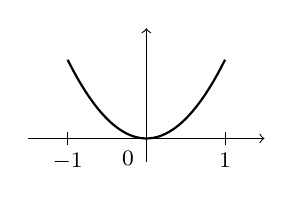
\begin{tikzpicture}[scale=1.0]
  \draw[->] (-1.5,0) -- (1.5,0);
  \draw[->] (0,-0.3) -- (0,1.4);
  \draw (-1,-0.08) -- (-1,0.08) node[below=4pt] {\footnotesize $-1$};
  \node[below left=1pt] at (0,0) {\footnotesize $0$};
  \draw (1,-0.08) -- (1,0.08) node[below=4pt] {\footnotesize $1$};
  \draw[domain=-1:1, smooth, variable=\x, thick] plot ({\x}, {\x*\x});
\end{tikzpicture}
\end{center}
\end{remarkbox}
\end{solution}
